\documentclass[tikz,border=10pt]{standalone}
\usepackage{tikz}
\usetikzlibrary{positioning, arrows.meta, fit, backgrounds}

\begin{document}
\tikzset{
	every node/.style={
		font=\Large,
		transform shape
	},
	every path/.style={
		line width=0.6pt
	}
}
	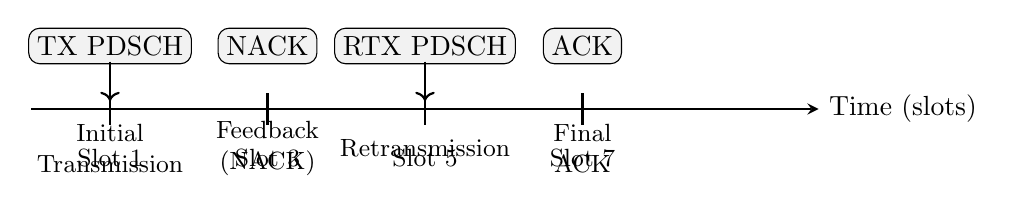
\begin{tikzpicture}[
		timeline/.style={thick,->,>=stealth},
		event/.style={draw,fill=black!5,rounded corners,inner sep=3pt},
		label style/.style={font=\small}
		]
		
		% Time axis
		\draw[timeline] (0,0) -- (10,0) node[right]{Time (slots)};
		
		% Initial transmission
		\draw[thick] (1,0.2) -- (1,-0.2) node[below=5pt,label style]{Slot 1};
		\node[event] at (1,0.8) {TX PDSCH};
		
		% ACK/NACK arrow
		\draw[->,thick] (1,0.6) -- (1,0.1);
		
		% NACK event (failed decode)
		\draw[thick] (3,0.2) -- (3,-0.2) node[below=5pt,label style]{Slot 3};
		\node[event] at (3,0.8) {NACK};
		
		% Retransmission
		\draw[thick] (5,0.2) -- (5,-0.2) node[below=5pt,label style]{Slot 5};
		\node[event] at (5,0.8) {RTX PDSCH};
		
		% ACK event
		\draw[->,thick] (5,0.6) -- (5,0.1);
		\draw[thick] (7,0.2) -- (7,-0.2) node[below=5pt,label style]{Slot 7};
		\node[event] at (7,0.8) {ACK};
		
		% Labels
		\node[align=center,font=\small] at (1,-0.5) {Initial \\ Transmission};
		\node[align=center,font=\small] at (3,-0.5) {Feedback\\ (NACK)};
		\node[align=center,font=\small] at (5,-0.5) {Retransmission};
		\node[align=center,font=\small] at (7,-0.5) {Final\\ ACK};
		
	\end{tikzpicture}



	
\end{document}
